\documentclass[12pt]{notes}

\usepackage{hyperref}

% Command for Questions
%\question{}

% Command for Notes
% \note{}

% Code to create a minipage where you can type in class notes. 
%%\begin{minipage}[l][2cm][c]{\textwidth}
%\begin{comment}

%\end{comment}
%%\end{minipage}


% Begin Document
%==============================================================================
\begin{document}
% Include the Title of the Handout
\ntitle{2.4: Simultaneous Inference and Important Considerations}
Simultaneous inference is when we want to conduct multiple tests of significance at the same time.

% Include Numbered Sections
\section{Why Simultaneous Inference?}
In handout 2.3, we conducted inference for parameters one at a time. We need to change our approach when looking at multiple parameters simultaneously. 

\question{(Groups) How and why do we need to change our approach when conducting simultaneous inference?}

(check out \href{https://xkcd.com/882/}{\textbf{\underline{this comic}}} for help).

\begin{minipage}[l][3cm][c]{\textwidth}
%\begin{comment}
\note{If we conduct several tests at the same level of significance, the probability of getting one false positive result (a type I) error becomes much higher than $\alpha$.}

\nspace
\note{As a result, we need to adjust the level of significance to account for a ``multiplicity'' of testing.}
%\end{comment}
\end{minipage}

\section{Bonferroni Adjustment}
Multiplicity:
\bi
\item Let $A_j =$ event that an individual $(1-\alpha)100\%$ CI does not contain the true value of $\beta_j.$
\item $P(A_0) = P(A_1) = \alpha \rightarrow$ Type I Error
\bi
\item $P(\text{NOT} A_j) = $ probability that an interval contains the true value of $\beta_j$.
\ei
\item \textbf{Bonferroni Inequality:} $P(\text{NOT} A_0 \text{ AND NOT } A_1) \ge 1 - P(A_0) - P(A_1)$ 
\ei

This means that if we conduct $g$ tests at a confidence level of $(1 - \frac{\alpha}{g})$, then we are guaranteed that overall level of confidence for all intervals \textit{considered jointly} will be at least $(1-\alpha)$, we call this the \textbf{Bonferroni adjustment}. 

\nspace
\bi
\item \textbf{Bonferroni Advantage:} Can be literally applied in \textit{any} situation requires a multiplicity adjustment, including simultaneous intervals for $\hat{Y}$ at multiple $X_h$ levels. 
\item \textbf{Bonferroni Disadvantage:} Can be overly conservative, producing inefficient (unnecessarily wide) intervals. 
\ei

\subsection*{Comparison of Simultaneous Intervals for $\hat{Y}$}
\bi
\item Confidence intervals (mean response)
\bi
\item Bonferroni
\[
\hat{Y} \pm t_{n-p}(1-\frac{\alpha}{2g})*s\{\hat{Y}_h\}
\]
\item Working-Hotelling (WH)
\[
\hat{Y} \pm W*s\{\hat{Y}_h\} \qquad \left(W = \sqrt{pF_{p, n-p}(1-\alpha)}\right)
\]

\begin{minipage}[l][2cm][c]{\textwidth}
%\begin{comment}
\note{Notice that the W-statistic does not consider $g$}
%\end{comment}
\end{minipage}

\bi
\item WH provides a ``confidence band'' for the entire regression line (all possible $X_h$ levels). 
\item This means the WH interval at any individual $X_h$ will be wider than the t-based confidence interval, but the WH intervals will eventually be narrower than Bonferroni confidence intervals if enough $X_h$ are considered. 
\ei
\ei

\item Prediction intervals (new response)

\bi
\item Bonferroni
\[
\hat{Y} \pm t_{n-p}(1-\frac{\alpha}{2g})*s\{\hat{Y}_{h (new)}\}
\]
\item Scheffe (chef-eh)
\[
\hat{Y} \pm S*s\{\hat{Y}_{h (new)}\} \qquad \left(S = \sqrt{gF_{g, n-p}(1-\alpha)}\right)
\]
\ei
\ei

\textbf{Rule of Thumb: Always pick the most efficient interval that guarantees your intended type I error ($\alpha$)}. 

\nspace

\begin{table}[H]
\centering
\caption{Summary of Methods for Simultaneous Intervals}
\begin{tabular}{|l|l|}
\hline
\textbf{Simultaneous Interval on:} & \textbf{Methods} \\ \hline
$\beta$'s & Bonferroni \\ \hline
Population means of $Y$ at multiple $X_h$ & Bonferroni or Working-Hotelling \\ \hline
Predictions for $Y$ at multiple $X_h$ & Bonferroni of Scheffe \\ \hline
\end{tabular}
\end{table}

\section{Inverse Prediction}
\textbf{Problem:} What is the value of $X_h$ necessary to achieve a specific value of $\hat{Y}.$ 

\nspace
\textbf{Solution:} solve for $X$.

\begin{align*}
\hat{Y} &= b_0 + b_1X_h \\
b_1X_h &= \hat{Y} - b_0 \\
X_h &= \frac{\hat{Y} - b_0}{b_1}
\end{align*}

\nspace \textbf{Problem:} Use $Y$ to predict values of $X$. 

\nspace \textbf{Solution:} DO NOT solve for X. 

\nspace \textbf{Why?}

\begin{itemize}
\item The least squares slope estimate of regression model that predicts $Y$ using $X$: $\rho\frac{SD\{Y\}}{SD\{X\}}$.
\item The least squares slope estimate of regression model that predicts $X$ using $Y$: $\rho\frac{SD\{X\}}{SD\{Y\}}$.
\item Notice that the slopes are NOT inverses of each other. 
\end{itemize} 

\begin{figure}[H]
\centering
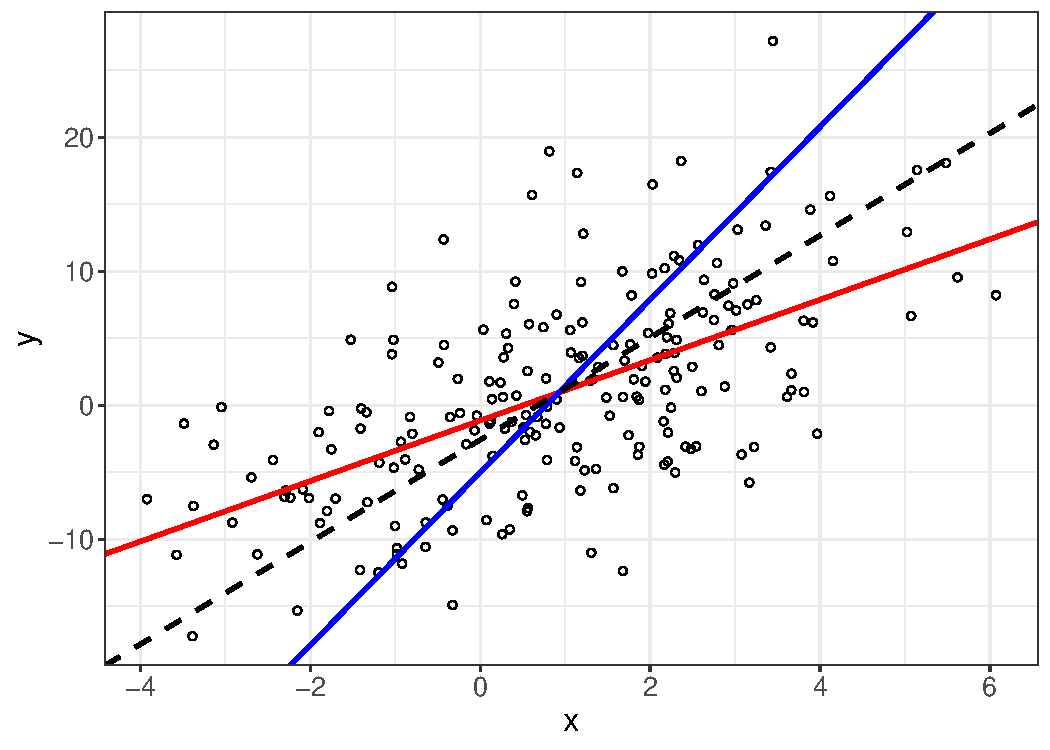
\includegraphics[width=0.6\textwidth]{figures/module2/sdline.pdf}
\caption{Scatterplot of points along with the regression line that uses X to predict Y (red), the regression line that uses Y to predict X (blue), the SD line (black). }
\end{figure}

\section{Regression through the Origin}
Sometimes we wish to force the regression line to go through the origin (i.e. the point (0,0)), making the theoretical linear model become
\[
Y_i = \beta_1X_{i, 1} + \epsilon_i
\]

\nspace
\question{When might regression through the origin be a good idea?} 

\begin{minipage}[l][3cm][c]{\textwidth}
%\begin{comment}
\note{\begin{itemize}
\item When the point (0,0) makes sense in the context of the data. 
\item When our sample size is small (avoiding an estimate of $\beta_0$ saves us one degree of freedom). 
\item If BOTH of the above conditions are not met, don't bother with regression through the origin. 
\end{itemize}
}
%\end{comment}
\end{minipage}

\nspace
Cautions for regression through the origin:
\bi
\item $\sum_ie_i$ not necessarily equal to 0 (residuals might be unbalanced)
\item $R^2$ can be negative, giving it a nonsensical interpretation\
\ei

\section{Cautions for Linear Regression}
\bi
\item Remedial measures may not fix violations of assumptions
\bi
\item May need to abandon OLS regression altogether
\ei
\item Interpretation: Sometimes the $X$ vs $Y$ relationship may look counterintuitive
\bi
\item May be the result of omitted predictors
\ei
\item $R^2$ can be abused
\bi
\item Higher $R^2 \rightarrow$ not always better model
\item Lower $R^2 \rightarrow$ does not mean there is no linear relationship 
\ei
\item Extrapolation
\bi
\item Linear model is only good for prediction/inference at or near the range of observed data points. 
\ei
\ei

\nspace
\question{(Individual) If I have created a linear model for prediction, would I WANT to extrapolate?}

\begin{minipage}[l][3cm][c]{\textwidth}
%\begin{comment}
\note{Slight extrapolations are usually not bad and even desirable. However, the farther you get away from the range of your observed data the more inappropriate your predictions will become. }
%\end{comment}
\end{minipage}

\begin{figure}[H]
\centering
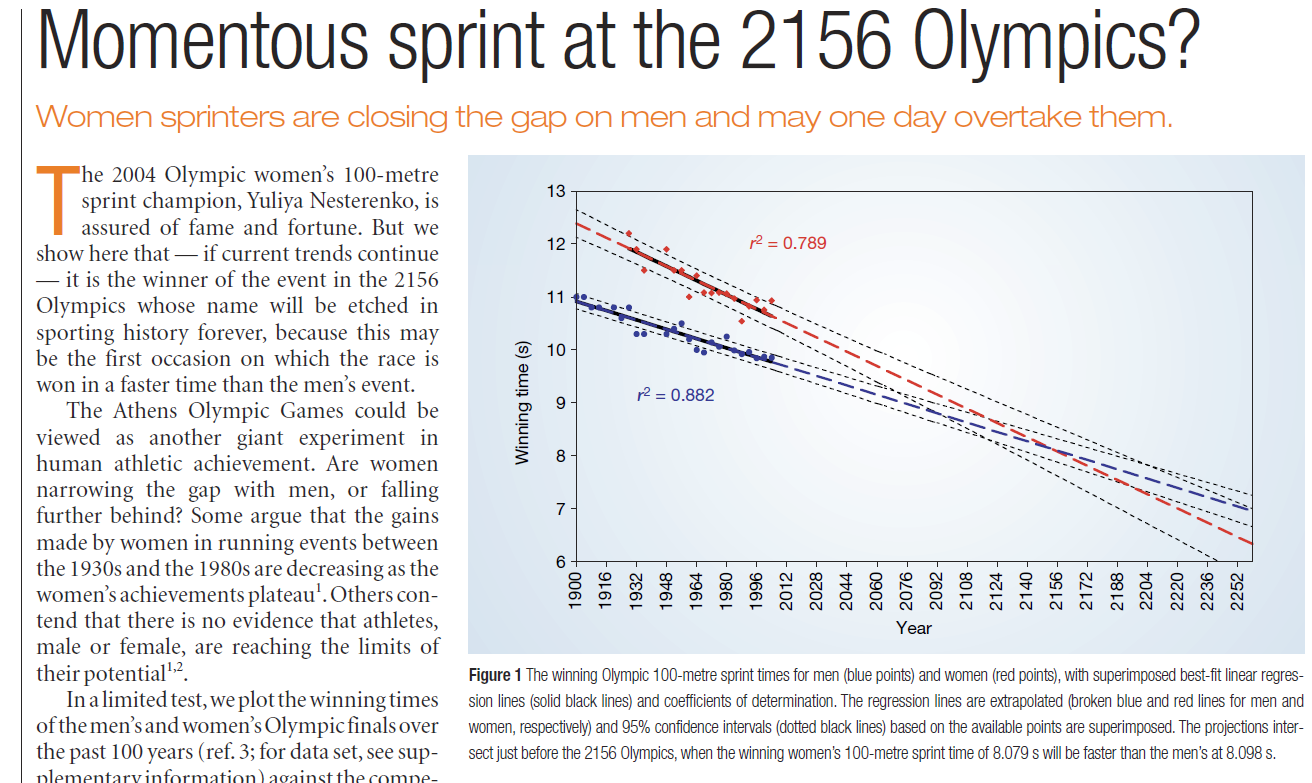
\includegraphics[width=\textwidth]{figures/module2/sprint.png}
\end{figure}













% End the Document
%==============================================================================
\end{document}